\section{Introduction}\label{sec:introduction}
A positive semidefinite contraction $H$ and its complement $I-H$ (the spectral shift of the title) have equally simple classical descriptions, but their quantum access costs can differ greatly. A coherent linear combination with the identity immediately gives a block encoding of $(I-H)/2$, but an algorithm that needs $I-H$ itself cannot discard the factor of two. When $H$ has a small eigenvalue, the corresponding eigenvalue of $I-H$ is close to the boundary of the unit disk. Because the circuit must be unitary for every input, this limits how accurately a circuit with finitely many queries can follow that eigenvalue on a whole interval.

This normalization problem appears explicitly in Orsucci and Dunjko's algorithms for positive-definite linear systems \cite[Section 4.3]{orsucci2021}, which need a normalized encoding of $I-\eta A$. We determine the query cost of the conversion when only a block encoding of $H$ is given and the spectrum of $H$ consists of a low band that shrinks to zero and a separated high band. The output is a reusable coherent operator, so the task differs from learning the matrix or preparing a single output state.

\subsection{Problem and results}
Fix $\rho>1$ and $0<c\leq1$. Let $\delta>0$ tend to zero with $\rho\delta<c$, and suppose
\[
 \spec(H)\subseteq[\delta,\rho\delta]\cup[c,1].
\]
We call $[\delta,\rho\delta]$ the low band and $[c,1]$ the high band. We want an output unitary whose designated block approximates $I-H$ in operator norm to error $\eta$, with normalization exactly one. Let $Q(\delta,\eta;\rho,c)$ be the minimum worst-case number of controlled calls to the input block encoding or its inverse. The converter must work for every matrix satisfying the promise and for every unitary completion of its block encoding; its gates may depend on $\delta,\rho,c,\eta$, but not on the unknown matrix. $Q$ counts one application of the output circuit; each reuse costs these queries again. Adaptive algorithms with a bounded number of queries are included, because their measurements can be deferred. Section~\ref{sec:model} states the model in full.

\paragraph{Fixed relative accuracy.}
Let $\eta=K\delta$ with fixed $K>0$. As $K$ decreases, the optimal query exponent changes in discrete steps at the thresholds
\[
 G_r(\rho)=\inf_{\substack{P\in\R[y],\ \deg P\leq2r\\ P\geq0\text{ on }\R}}
                \max_{1\leq y\leq\rho}|P(y)-y|,
 \qquad r=0,1,2,\ldots,
\]
the least uniform error on $[1,\rho]$ of a polynomial of degree at most $2r$ that approximates $y$ and is nonnegative on all of $\R$. Our first main result computes these thresholds explicitly and determines the optimal query count for every $K$; we call the resulting sequence of costs the query staircase, and the range $G_\ell\leq K<G_{\ell-1}$ its $\ell$th tier. If $\ell=\min\{r:G_r\leq K\}\geq1$, then
\[
 Q(\delta,K\delta;\rho,c)=\Theta(\delta^{-1+1/(2\ell)}).
\]
The constants may depend on the fixed parameters; at an equality $K=G_\ell$ the cheaper order holds. In the coarse tier $K\geq G_0=(\rho-1)/2$, the cost is $\Theta(\log(1/\delta))$ when $c<1$, and $\Theta(1)$ when the high band is the single point $\{1\}$. See Theorems~\ref{thm:staircase} and~\ref{thm:thresholds} and Figure~\ref{fig:overview}. In contrast, a spectrum contained in two known points $0<a<b\leq1$ with $(1-a)(1-b)\leq a+b$ admits exact conversion with two queries (Proposition~\ref{prop:two-point}), but no finite-query converter is exact on a nonempty interval at any normalization below two (Proposition~\ref{prop:no-exact}).

\paragraph{Parity.}
A single real quantum singular value transformation (QSVT) of definite parity implements a bounded even or odd polynomial of $H$. Even polynomials have their own optimal staircase, governed by the same approximation problem with $P$ also required to be even; we denote its thresholds by $F_r$. We prove that $F_1$ and $F_2$ coincide:
\[
 F_1(\rho)=F_2(\rho)=\frac{(\rho-1)^2}{8(\rho+1)}.
\]
So the even staircase skips the tier with exponent $3/4$. At $\rho=2$ and $\eta=\delta/32$, even polynomials need $\Theta(\delta^{-5/6})$ queries, whereas arbitrary coherent circuits need $\Theta(\delta^{-1/2})$; the even upper bound uses an explicit degree-six polynomial that is positive on all of $\R$ and bounds $F_3(2)$ from above; we do not compute $F_3(2)$ itself. Odd polynomials need $\Theta(\delta^{-1}\log(1/\delta))$ queries at every fixed $K>0$ (Theorem~\ref{thm:even-staircase} and Proposition~\ref{prop:odd-optimal}). These restrictions concern a single definite-parity transform, not arbitrary compositions of QSVT circuits. The unrestricted upper bounds use generalized quantum signal processing (GQSP), which loses no normalization.

\paragraph{Accuracy shrinking with $\delta$.}
We now let $K$ depend on $\delta$. For every fixed $\beta>0$, uniformly over $0<K\leq\delta^\beta$,
\[
 Q(\delta,K\delta;\rho,c)
 =\Theta_{\rho,\beta}\bigl(\delta^{-1}\log(1/K)\bigr).
\]
For the full spectral interval $[\delta,1]$, the corresponding order is
$\Theta_\beta(\delta^{-1}\log(1/\eta))$ when $0<\eta\leq\delta^{1+\beta}$ (Theorem~\ref{thm:joint-matched}). In the intermediate regime, where $K\to0$ and $\log(1/K)=o(\log(1/\delta))$, let $r=\min\{j:G_j\leq K\}$. Our bounds, uniform in $r$, have the same power $\delta^{-1+1/(2r)}$, with prefactors $r(G_{r-1}-K)^{1/r}$ in the lower bound and $r^3$ in the upper bound. If $K\leq(1-\gamma)G_{r-1}$ for a fixed $\gamma\in(0,1)$, their ratio is at most $O(r^2)=O(\log(1/K)^2)$; this includes $K=G_r$ for large $r$. Near $G_{r-1}$ the lower bound keeps the factor $(G_{r-1}-K)^{1/r}$. In the intermediate regime we do not determine the cost up to a constant factor (Corollary~\ref{cor:joint-near-match}).

\paragraph{A linear program.}
Finally, we compare access models on a sparse linear program (LP) with three variables and two equality constraints, at a primal--dual point exactly on the central path. Its normal matrix is $H_t=A_tA_t^T$, with hidden $t\in[\delta,\rho\delta]$ and condition number $\Theta(\delta^{-1})$. Preparing the normalized \emph{dual} Newton direction to a fixed trace distance costs $\Theta(\delta^{-1})$ queries to the specified block encoding of the normal matrix and $\Theta(\delta^{-1/2})$ queries to that of the factor $A_t$, even when queries to the unitary that prepares the right-hand side are counted (Theorem~\ref{thm:lp-state}). Converting a block encoding of $H_t$ alone into a reusable unit-normalized block encoding of $I-H_t$ costs as in the staircase for every $\ell\geq1$ and $\Theta(\delta^{-1}\log(1/\eta))$ for $\eta\leq\delta^{1+\beta}$ with fixed $\beta>0$, whereas two queries to the factor give $I-H_t$ exactly. Because the spectral projectors of $H_t$ are public, the coarse tier needs no queries (Theorem~\ref{thm:lp-compiler}). These results concern the specified quantum oracles; the primal Newton (affine-scaling predictor) direction is public, and digital access to matrix entries reveals $t$. They are not lower bounds for solving the LP or for a complete quantum interior-point method.

\begin{figure}[t]
\centering
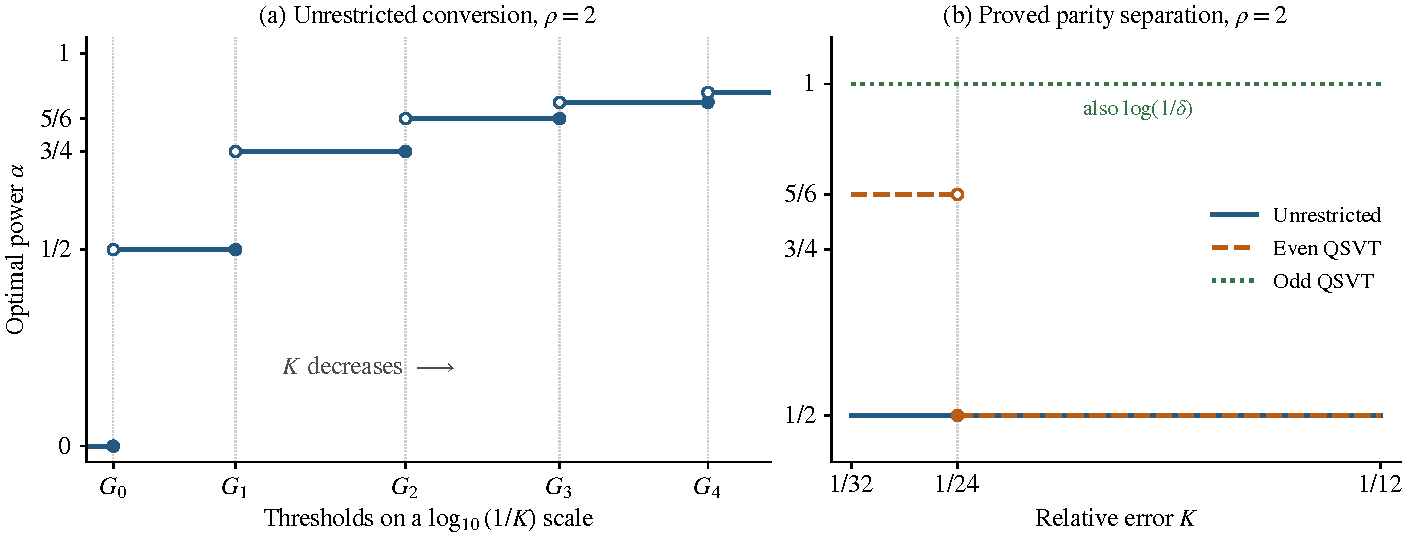
\includegraphics[width=\textwidth]{figures/query-overview.pdf}
\caption{Optimal query powers for fixed relative accuracy, with $\rho=2$. Left: the unrestricted exponent $\alpha$ in $Q=\delta^{-\alpha+o(1)}$ as $K$ decreases. At a threshold, a filled marker selects the cheaper tier; an open marker excludes the more expensive one. The coarse exponent zero includes a logarithmic cost for $c<1$. Right: the proved parity comparison on $1/32\leq K\leq1/12$. Because $F_1=F_2=1/24$, the even exponent jumps from $1/2$ to $5/6$; the odd class also has a logarithmic factor. The plot does not determine $F_3$. Threshold locations on the left are numerical evaluations of the exact formula in Theorem~\ref{thm:thresholds}; all complexity statements are proved.}\label{fig:overview}
\end{figure}

\subsection{Related work and contributions}
Quantum signal processing (QSP) and QSVT provide the tools we use to implement bounded polynomials. Gily\'en, Su, Low, and Wiebe \cite{gilyen2019} establish general singular value transformations, bounded approximations of the sign function, uniform amplification, and lower bounds for eigenvalue transformations from pairs of inputs. Low and Chuang \cite{low2017} develop uniform spectral amplification and track its normalization. Motlagh and Wiebe's GQSP \cite{motlagh2024} removes the usual definite-parity restriction by synthesizing bounded polynomials on the unit circle. We use these results, including a reduction to Laurent polynomials that works for arbitrary completions of the input block encoding; neither removing the parity restriction nor the generic amplification upper bound is our contribution. We count oracle queries and allow exact oracle-independent gates. Classical computation of phases and finite-precision circuit synthesis are separate questions; Haah \cite{haah2019} gives a rigorous algorithm for computing such phase decompositions and analyzes its cost.

The relation between analog quantum queries and trigonometric polynomials is known. Bessen \cite{bessen2004} uses it to compare real-valued query models, and Laneve \cite{laneve2026} characterizes QSP through state conversion and adversary feasibility. Our reduction to a scalar oracle is an instance of this polynomial method. What we add is the combination of two constraints: the circuit is unitary for every value of the scalar oracle, but it must be correct only on an interval that shrinks with $\delta$. After the rescaling $x=\delta y$ and division by $\delta$, any limit of the low-degree Taylor polynomials of $1-\operatorname{Re}q$, where $q$ is the output amplitude, must be nonnegative on all of $\R$. This leads to the extremal problem that defines $G_r$ and gives lower bounds for all coherent circuits, not only single QSP sequences. The pairwise square-root lower bound alone does not give the higher tiers.

In constrained polynomial approximation, Taylor \cite{taylor1968} studies restricted ranges, Lewis \cite{lewis1973} treats convex constraints, and Campos-Pinto, Charles, and Despr\'es \cite{campos2019} develop algorithms for positive polynomial approximation. Fawzi, Saunderson, and Parrilo \cite[Sections 3.1--3.2 and Appendix A, Lemma 1]{fawzi2017} study globally nonnegative interpolation of affine targets at finite nodes and use supporting tangents of Chebyshev polynomials; our threshold problem instead minimizes the uniform error on $[1,\rho]$. Its solution uses the classical Chebyshev inequality outside an interval, as stated for example by Bos, Ma'u, and Waldron \cite[Proposition 2.1]{bos2020}; our quantitative lower bounds also use the classical Fej\'er--Riesz factorization. The odd upper bound uses known sign approximations from QSVT, with antecedents in approximation theory by Eremenko and Yuditskii \cite{eremenko2007,eremenko2011}; the resulting degree of order (inverse gap) times $\log(1/\text{error})$ is not new. We use it for matching odd-polynomial bounds, with an elementary lower bound that uses correctness only on the low band.

Sarkar and Yoder \cite{sarkar2023} prove qualitative density results for QSP-related polynomial families with range constraints inside and outside the approximation interval, under necessary matching conditions at the endpoints, and study approximation of step functions; we ask for quantitative degree thresholds and coherent query costs as the correctness interval shrinks.

A particularly close recent work is that of Dong, Larsen, Lin, and Sarkar \cite{dong2026}. They formulate the design of QSP polynomials with prescribed parity as minimax fitting on a subset subject to a global bound on the modulus, study Remez methods with active constraints, and introduce a nonlinear Fourier retraction that restores feasibility without increasing the degree. Their work shows why bounds checked at sampled points are not enough, especially near the boundary of the feasible set. We address an analytic asymptotic question for one target and one spectral promise: exact limiting thresholds, optimal query powers over all circuits, and constructions that attain the threshold error. We prove on continuous domains that these constructions are bounded by one on $[-1,1]$ and that their error does not exceed the threshold, even at the points where the limiting error equals it; numerical plots are only illustrations. We do not propose a general minimax solver or a phase-synthesis algorithm.

In their Section 4.3, Orsucci and Dunjko \cite{orsucci2021}, our most direct motivation, also invoke QSVT lower bounds against generic amplification and give constructions from sparse matrix values for diagonally dominant matrices and for local sums of positive semidefinite terms; our analysis of plain block encodings does not resolve their question of a general construction from sparse matrix values. Their factor-based algorithms also explain square-root improvements in the condition number and the associated requirement on support overlap. Factor and sum-of-squares access are also central to the spectral amplification of King et al.\ \cite{king2026}. Somma and de Wolf \cite{somma2026} prove joint lower bounds for guided ground-state energy estimation and state preparation, including sum-of-squares access, under assumptions on guide overlap and dimension. Their tasks and hypotheses differ from ours, and we do not claim that their bounds apply here. Our state upper bounds for the LP use standard amplitude estimation \cite{brassard2002}.

Our contributions are: explicit formulas for the thresholds $G_r$ of the globally nonnegative approximation problem, and the complete fixed-accuracy query staircase for converting $H$ to $I-H$; the equality $F_1=F_2$ and the resulting sharp parity separation; lower bounds for interval spectra, uniform in the accuracy, that match the amplification cost when $K\leq\delta^\beta$, and a bound on the remaining gap at intermediate accuracy; and an explicit exactly central LP with fully specified oracles and matching bounds under access to the normal matrix and to its factor. To our knowledge, this combination of exact thresholds, constructions that attain the threshold error, and optimal query exponents for converting $H$ to $I-H$ has not appeared in the cited literature. This claim concerns the stated problem and theorems, not the underlying techniques of synthesis, approximation, or factor access.

\subsection{Organization}
Section~\ref{sec:model} connects block encodings to bounded polynomials and represents circuits with a scalar oracle by trigonometric polynomials. Section~\ref{sec:exact} contrasts finite known spectra with interval promises. In Section~\ref{sec:fixed}, global unitarity forces a nonnegative Taylor limit, Chebyshev growth outside an interval gives the thresholds, and a polynomial gate pinned to one where the approximation error equals $+G_r$ turns the extremal polynomial of the threshold problem into a converter bounded by one with error at most the threshold. Section~\ref{sec:joint} replaces fixed-order compactness by uniform Taylor estimates and an independent Fej\'er--Riesz argument, and controls the pinned construction when the order grows. Section~\ref{sec:lp} treats the LP. Section~\ref{sec:conclusion} lists open questions, and Appendix~\ref{app:reproduce} describes how to reproduce Figure~\ref{fig:overview} and build the source.
